        \clearpage
        \begin{figure*}[ht]
            \pdfbookmark[2]{ID 07}{figure_id_07}
        	\centering
            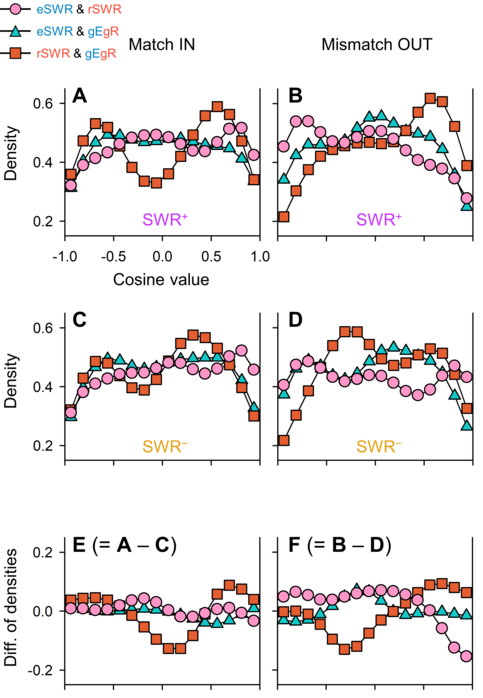
\includegraphics[width=0.5\textwidth]{./src/figures/.png/Figure_ID_07.png}
        	\caption{\textbf{
Neural trajectory directions of SWR based on encoding and retrieval states
}
\smallskip
\\
\textbf{\textit{A--B}} Kernel density estimation (KDE) distribution of $\protect\overrightarrow{{\mathrm{eSWR^+}}} \cdot \protect\overrightarrow{{\mathrm{rSWR^+}}}$ (\textit{pink circles}), $\protect\overrightarrow{{\mathrm{eSWR^+}}} \cdot \protect\overrightarrow{{\mathrm{g_{E}g_{R}}}}$ (\textit{blue triangles}), and $\protect\overrightarrow{{\mathrm{rSWR^+}}} \cdot \protect\overrightarrow{{\mathrm{g_{E}g_{R}}}}$ (\textit{red rectangles}) in Match In (\textit{A}) and Mismatch OUT task (\textit{B}). \textbf{\textit{C--D.}} The corresponding distributions of $\mathrm{SWR^-}$ instead of those of $\mathrm{SWR^+}$ in \textit{A--B}. \textbf{\textit{E--F.}} The differences in distributions of $\mathrm{SWR^+}$ and $\mathrm{SWR^-}$, highlighting the SWR components (\textit{E} = \textit{C} $-$ \textit{A}; \textit{F} = \textit{B} $-$ \textit{D}). Note the biphasic distributions of $\protect\overrightarrow{{\mathrm{rSWR^-}}} \cdot \protect\overrightarrow{{\mathrm{g_{E}g_{R}}}}$, indicating neural fluctuation betwen the encoding and retrieval states during the Sternberg task. Additionally, in Mismatch OUT task, inverse directionality between $\protect\overrightarrow{{\mathrm{eSWR^+}}}$ and $\protect\overrightarrow{{\mathrm{rSWR^+}}}$ (\textit{pink circles}) was found, though not in Match IN task \textbf{\textit{E--F}}). Last, shifts from the retrieval to encoding states were observed for SWR components both in Match IN and Mismatch OUT tasks (\textit{red rectangles} in \textit{E--F}).
}
% width=0.5\textwidth
        	\label{fig:07}
        \end{figure*}
